\documentclass[../main.tex]{subfiles}
\graphicspath{{\subfix{../images/}}}
\begin{document}

%%%%%%%%%%%%%%%%%%%%%%%%%%%%%%%%%%%%%%%%%%%%%%%%%%%%%%%%%%%%%%%%%%%%%%%%%%%%%%%%
\section{Основы работы с мультиметром}
\index{Электроника!Мультиметр}

Мультиметр -- незаменимый прибор, с его помощью можно узнать сопротивление
резистора, измерить напряжение, произвести проверку на проводимость
(``прозвонка''), узнать цвет и полярность светодиода и многое другое.

На рис. \ref{fig:multimeter-example} показан один из вариантов мультиметра.

\begin{figure}[ht]
  \centering
  \caption{Пример мультиметра.}
  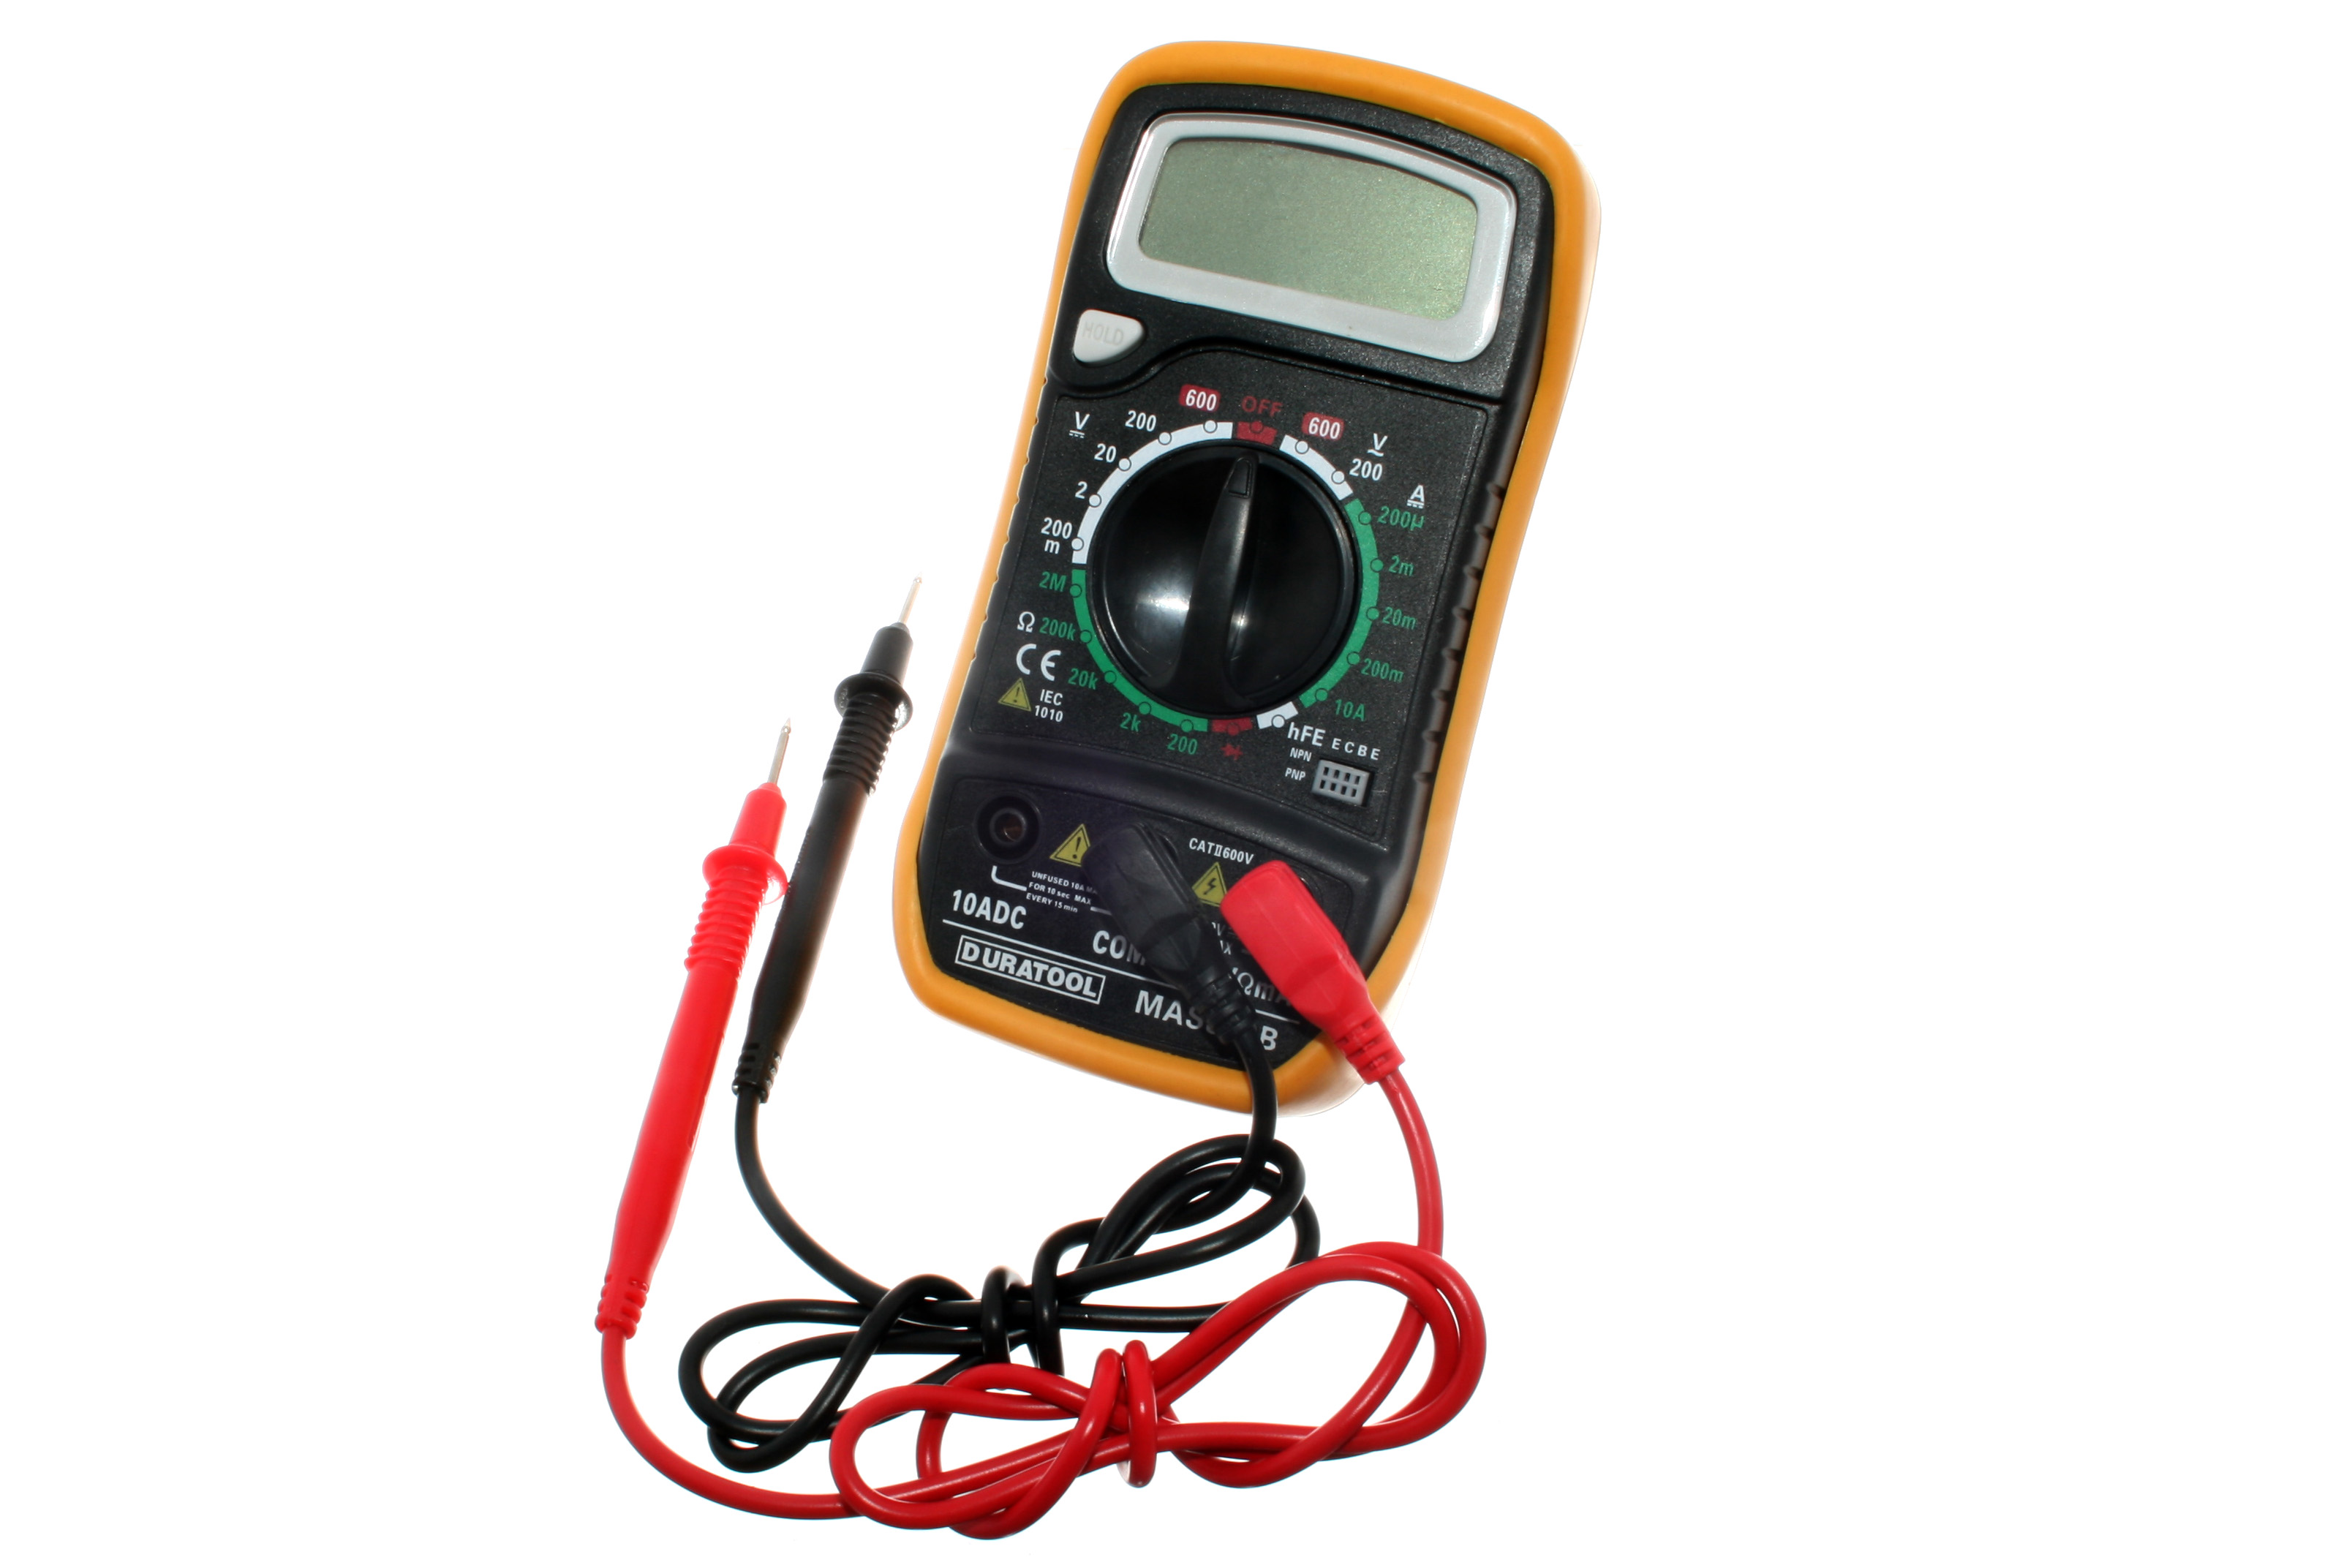
\includegraphics[width=12cm]{Digital_Multimeter}
  \label{fig:multimeter-example}
\end{figure}

Далее приведена таблица на которой отражены основные символы, встречающиеся на
корпусе прибора, необходимые для работы с мультиметром:

\begin{tabular}{| m{8em} | m{22em} |}
  \hline
  \textbf{Обозначение} & \textbf{Описание} \\
  \hline
  V$\sim$ & Измерение напряжения переменного тока. \\
  \hline
  mV$\sim$ & Измерение напряжения переменного тока, милливольты (мВ.) \\
  \hline
  V\Beam & Измерение напряжения постоянного тока. \\
  \hline
  mV & Измерение напряжения постоянного тока, милливольты (мВ.) \\
  \hline
  A\Beam & Измерение постоянного тока. \\
  \hline
  A$\sim$ & Измерение переменного тока. \\
  \hline
  $\Omega$ & Измерение сопротивления. Как правило, доступны следующие диапазоны:
  ``2k'' (2000 Ом), ``20k'' (20000 Ом), ``200k'' (200000 Ом) и ``2M'' (два
  мегаома, или два миллиона Ом.)\\
  \hline
  HOLD & ``Заморозить'' текущее показание на дисплее. \\
  \hline
  \esymbol{diode} & Тестирование диодов. \\
  \hline
  Hz   & ``Hertz'', Герцы -- измерение частоты. \\
  \hline
  \esymbol{capacitor} & Измерение ёмкости. \\
  \hline
  \soundWaveIcon{} & Измерение целостности цепи (так называемая ``прозвонка''.) \\
  \hline
  hFE & ``\textbf{H}ybrid parameter \textbf{f}orward current gain, common
  \textbf{e}mitter'' -- режим тестирования транзисторов. \\
  \hline
\end{tabular}

%% TODO: Добавить описание функций мультиметра.

\experiment{0} { Попробуйте померять с помощью мультиметра сопротивление
  резисторов, соединяя их последовательно и параллельно через макетную плату.
  Как меняется сопротивление собранной цепи? }

\experiment{1} { Померяйте сопротивление других проводников -- например, проводов
  для макетной платы Arduino, металлических предметов. Какое у них
  сопротивление?}

\experiment{2} { Известно, что графит является проводником. Померяйте
  сопротивление графитового стержня в карандаше.  Также попробуйте на листе
  бумаги нарисовать жирную графитовую линию и померяйте её сопротивление.  Какое
  сопротивление вы видите? }

\end{document}
